\section{fireMIP}
\pgfdeclareimage[width=1.0\paperwidth]{header-image}{header_images/red_lightn}



\begin{frame}[label = fireModels]
	\frametitle{fireModels}
	\foreach \x in {1, 2, 3, 4} {
		\only<\x> {
			\includegraphics[width=10cm]{images/fireModelTypes/pp\x.png}
	}}
	
\end{frame}

\begin{frame}[label = intro]
	\frametitle{FireMIP benchmarking}
	\framesubtitle{Benchmark Datasets}
	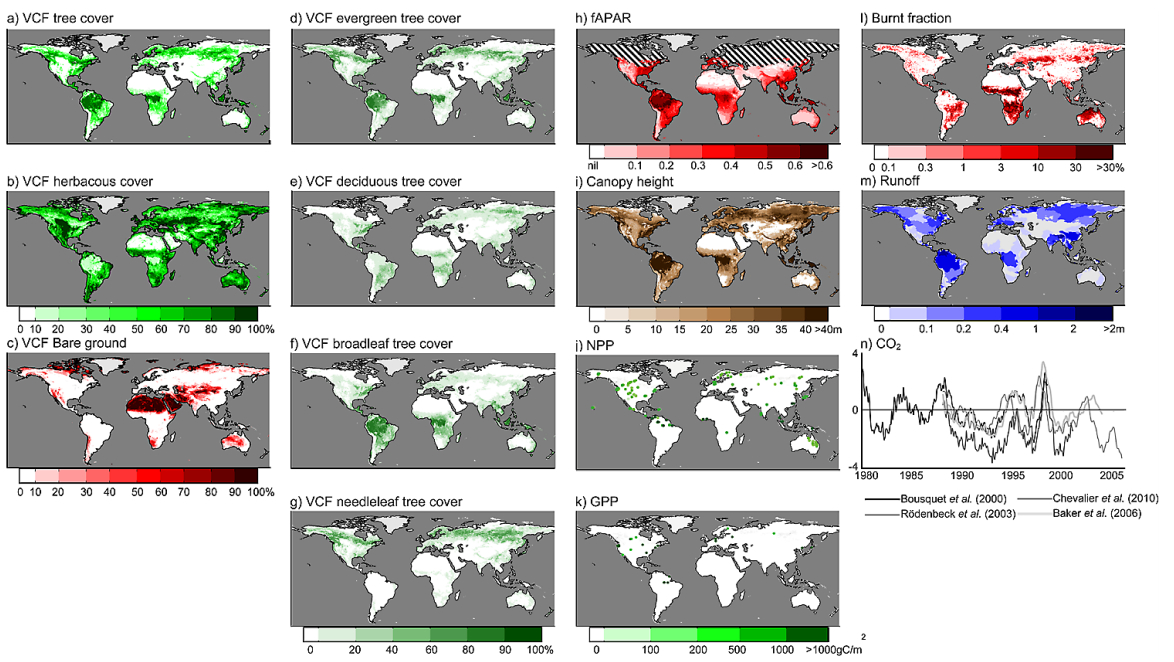
\includegraphics[width=10cm]{images/BenchmarkDatasets.JPG}
\end{frame}

\begin{frame}[label = intro]
	\frametitle{FireMIP benchmarking}
	\framesubtitle{Fire Benchmark Datasets}
	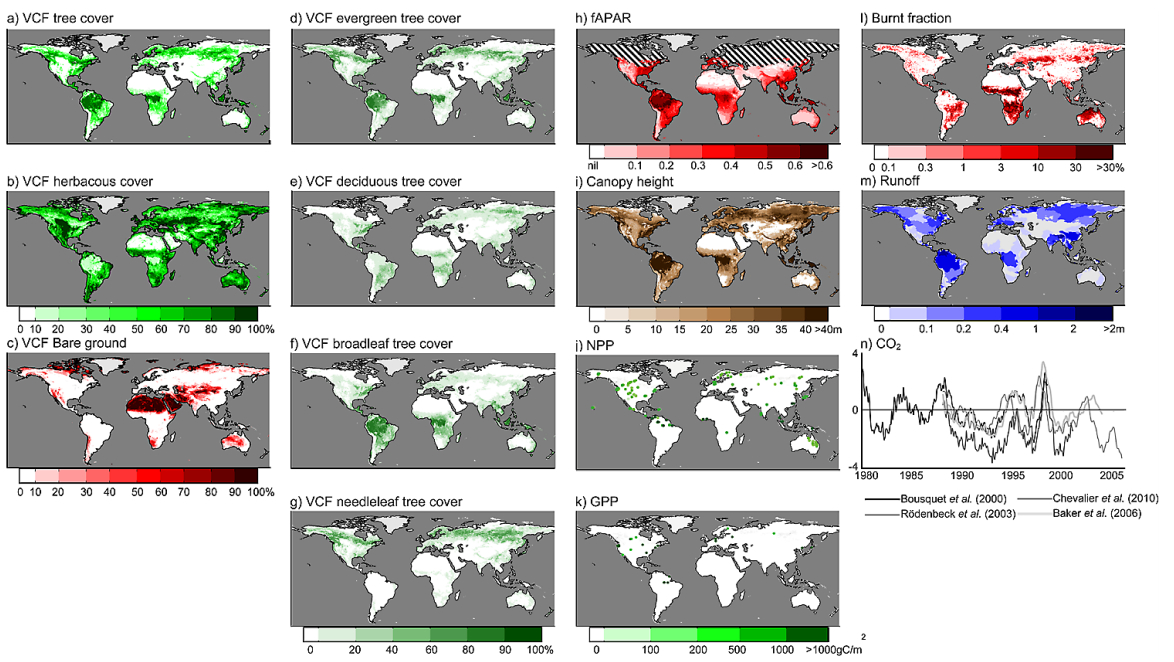
\includegraphics[width=10cm]{images/BenchmarkDatasets.JPG}
\end{frame}